\section{Dynamik}
$\implies$ Ursache der Bewegung
\subsection{Kraft/Masse}
\begin{def*}[ note = Kraft , index = Kraft ]
	\dots Wirkung!
\end{def*}
\begin{bsp*}
	\begin{itemize}
		\item Gewicht heben
		\item Deformation (Messung!)
		\item Bewegung
	\end{itemize}
\end{bsp*}
\begin{def*}[ note = Masse , index = Masse ]
	\enquote{Trägheit} (\enquote{\dots schwieriger in Bewegung zu setzen})
\end{def*}
Kraft: Vektor! \\
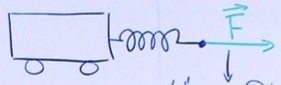
\includegraphics{Bild19} \\
Länge, Richtung, Angriffspunkt

\subsection{Die Newtonschen Prinzipien (1686)}
\begin{gather*}
	\underbrace{\vec{F}}_{\text{Ursache}} = \underbrace{m \cdot \vec{a}}_{\text{Wirkung}} \\
	[F] = \si{\kilo\gram\metre\per\second\tothe{2}} = \si{\newton} \quad ( \text{Newton} )
\end{gather*}
$\implies$ 2. Newtonsche Prinzip (Axiom) (Aktionsprinzip) \\
Anwendung: \\
\begin{itemize}
	\item Mann kennt Kraft $\implies$ Beschleunigung + Bahn berechnen
	\item Ich sehe Beschleunigung $\implies$ Was für Kräfte wirken
\end{itemize}
\subsubsection{1. Newtonsches Prinzip (Trägheitsprinzip)}
kräftefreie Körper ( $\vec{F} = \vec{0}$ , $\sum_i \vec{F_i} = \vec{0}$ )
\begin{itemize}[ label = $\rightarrow$ ]
	\item Körper in Ruhe (ist + bleibt)
	\item bewegt sich mit konst. Geschwindigkeit $\vec{v} =$ konst.
\end{itemize}
$\implies$ Bewegungszustände

\subsubsection{Newtonsches Prinzip (Reaktionsprinzip)}
(action = reactio) \\
Kräfte rühren immer von Wechselwirkungen (WW)
\begin{bsp*}[note = Feder]
	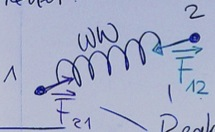
\includegraphics{Bild20}
	\[ \vec{F_{21}} = -\vec{F_{12}} \]
	Reaktionspartner $\rightarrow$ greifen immer an verschiedenen Körper an
\end{bsp*}
\begin{rep*}[ note = Dynamik ]
	Kraft: erzeugt Bewegung \\
	Masse: Trägheit \\
	Newtonsche Prinzipien \\
	\begin{enumerate}
		\item kräftefreier Körper: $\vec{v} =$ konst. (z.B. $\vec{v} = \vec{0}$)
		\item $\vec{F} = m \vec{a}$ Ursache \& Wirkung
		\item Kräfte rühren \textbf{immer} von WW her \\
			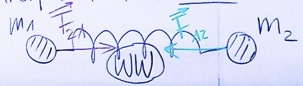
\includegraphics{Bild21} \\
			$\vec{F_{21}} = -\vec{F_12}$
	\end{enumerate}
\end{rep*}
\begin{bsp*}[ note = Hammer \& Nagel ]
	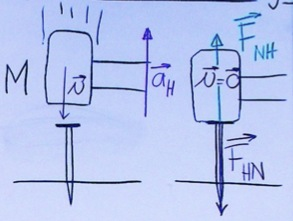
\includegraphics{Bild22}
	\begin{enumerate}[start = 2]
		\item $\vec{F_{NH}} = M \vec{a_H}$
		\item $\vec{F_HN} = -\vec{F_{NH}}$
	\end{enumerate}
\end{bsp*}

\subsection{Arten von Kräften}
\subsubsection{Gravitationskraft}
(Anziehung von Massen) \\
auf Erdoberfläche Gewichtskraft $\vec{G}$ \\
\begin{tabular}{ll}
	Betrag:			&$mg$ \\
	Richtung:			&zum Erdmittelpunkt \\
	Angriffspunkt:	&Schwerpunkt \\
	Reaktionspartner:	&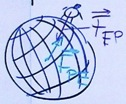
\includegraphics{Bild23}
\end{tabular}

\subsubsection{Elektromagnetische Kräfte}
(Anziehung / Abstossung von Ladungen)
\begin{itemize}[ label = $\rightarrow$ ]
	\item Coulombkraft (elektrische Kraft; verschiedene Erscheingungsformen)
	\item magnetische Kraft
	\item Lorentzkraft
\end{itemize}

\subsubsection{starke Kraft}
\begin{itemize}[ label = $\rightarrow$ ]
	\item Stabilität der Atomkeime
\end{itemize}

\subsubsection{schwache Kraft}
\begin{itemize}[ label = $\rightarrow$ ]
	\item Radioaktivität
\end{itemize}

\subsection{Coulombkraft und ihre Erscheinungsformen}
\begin{itemize}
	\item elastische Kräfte im festen Körpern (Kohäsion)
	\item Berührungskräfte - Die Normalkraft
		\begin{bsp*}[ note = Quader auf Tisch in Ruhe ]
			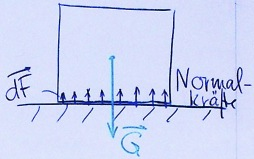
\includegraphics{Bild24}
			\begin{gather*}
				\sum \vec{F_a} = \vec{0} \\
				\implies \vec{G} + \sum \vec{\dd F} = \vec{0}
			\end{gather*}
		\end{bsp*}
\end{itemize}

\subsubsection{Coulombgesetz}
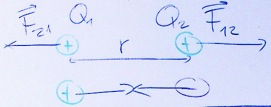
\includegraphics{Bild25}
\[ F_{21} = F_{12} = \frac{1}{4 \pi \epsilon_0} \frac{Q_1 Q_2}{r^2} \]
elektrische Feldkonstante $\epsilon_0 = \SI{8.85e-12}{\ampere\second\per\volt\metre}$

\subsubsection{Kraftgesetz zwischen zwei Atomen}
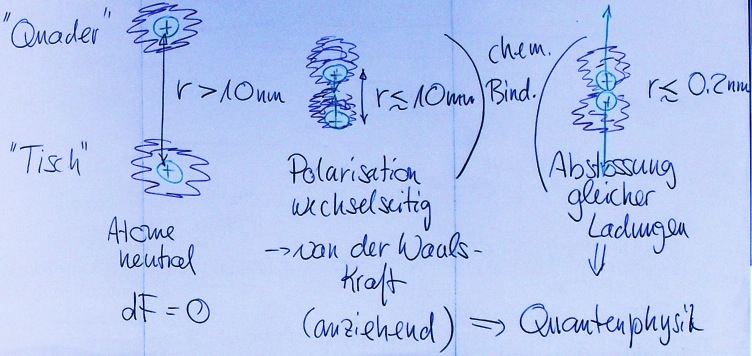
\includegraphics{Bild26}

\subsubsection{Kraftkurve}
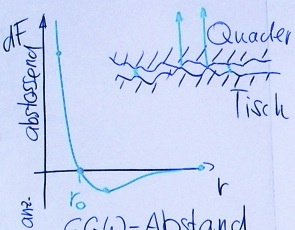
\includegraphics{Bild27} \\
GGW-Abstand (chemische Bindung)

\subsection{Reibungskräfte}
(parallel zur Berührungsfläche)

\subsubsection{Haftreibung}
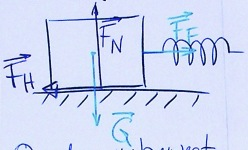
\includegraphics{Bild28} \\
Quader unbewegt \\
\[ \vec{F_H} = -\vec{F_F} \]

maximale Haftreibung:
\[ F_H \leq \underbrace{\mu_H}_{\text{Haftreibungszahl}} F_N \]

\subsection{Gleitreibung \texorpdfstring{$\vec{F_R}$}{F_R}}
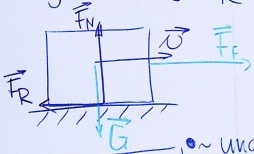
\includegraphics{Bild29}
\begin{itemize}
	\item Richtung: versucht immer Relativbewegung zu bremsen.
	\item unabhängig von $v$
\end{itemize}
\[ F_R = \mu_G \cdot F_N \]

\subsection{Kraftstösse}
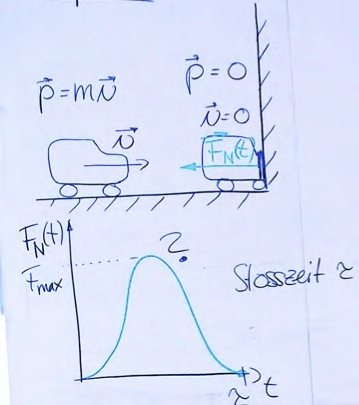
\includegraphics{Bild30}
\begin{rep*}
	Atomic Force Microscope (AFM) \\
	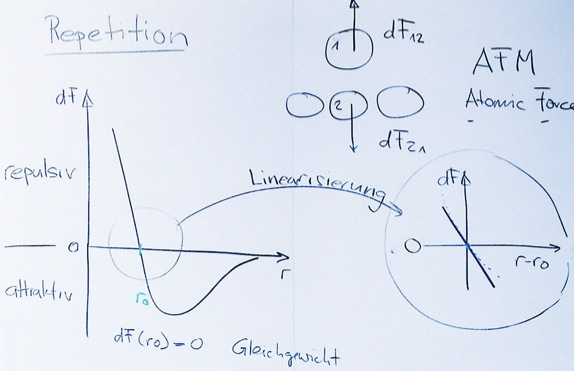
\includegraphics{Bild31}
	\[ \dd F =  -D ( r - r_0 ) = -\underbrace{D}_{\text{Federkonstante}} \cdot \underbrace{x}_{\text{Auslenkung}} \]
	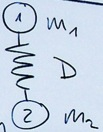
\includegraphics{Bild32}
	\[ D( \ce{O2} ) \approx \SI{1200}{\newton\per\metre} \]
\end{rep*}
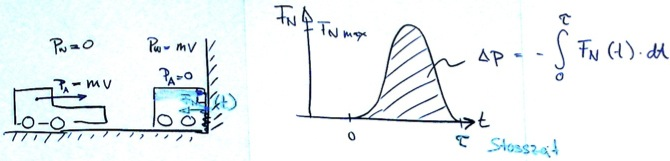
\includegraphics{Bild33}
\[ \Delta p = -\int_0^\tau F_n(t) \cdot \dd t \]
$\tau$ Stosszeit \\
kleine Kräfte $F_N$:
\begin{itemize}
	\item wenn $\tau$ gross
	\item wenn $\Delta p$ klein
\end{itemize}

\subsubsection{Experiment}
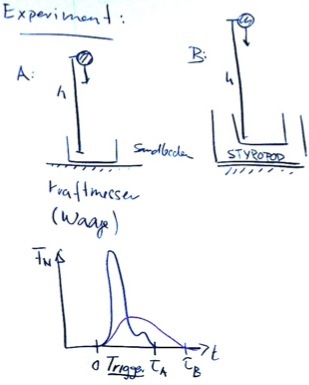
\includegraphics{Bild34}

\subsubsection{Vereinfachung}
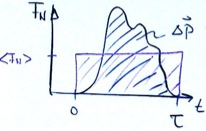
\includegraphics{Bild35}
\[ \Delta \vec{p} = m \vec{v} = - \scal{\vec{F_N}} \tau = - \int_0^\tau F_N(t) \dd t \]

\subsection{Das Drehmoment}
\begin{def*}[ note = Drehmoment , index = Drehmoment ]
	\[ \vec{M_0} = \vec{r} \times \vec{F} \]
\end{def*}
(Hebelgesetz) \\
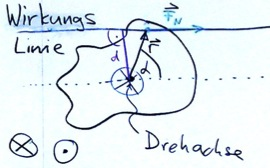
\includegraphics{Bild36}
\[ M_0 = r \cdot F_N \cdot \sin \alpha = \dd F_N \]
Rechte-Hand-Regel: \\
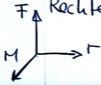
\includegraphics{Bild37}

\subsection{Gleichgewicht starrer Körper}
keine Bewegung:
\begin{gather*}
	\sum \vec{F_i} = 0 \quad \text{Translation} \\
	\sum \vec{M_i} = 0 \quad \text{Rotation}
\end{gather*}

\subsection{Der Schwerpunkt SP}
\begin{def*}[ note = Schwerpunkt , index = Schwerpunkt ]
	\[ \vec{r_s} = \frac{\sum \overbrace{m_i}^{\text{Massenelement}} r_i}{\sum m_i} \]
\end{def*}
gewichtetes  Mittel aller Orte der Körpermassen und ist der Angriffspunkt der Gewichtskraft \\
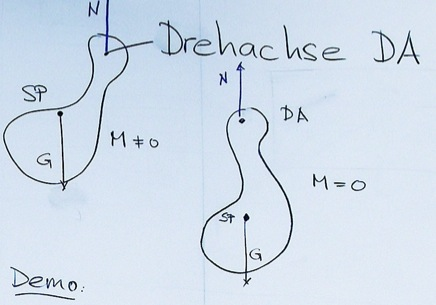
\includegraphics{Bild38}

\subsubsection{Denkexperiment Spazierstock}
Schwerpunkt des \\
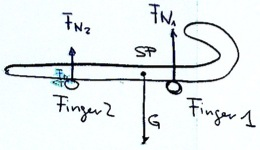
\includegraphics{Bild39} \\
wenn $F_{R_1} > F_{R_2}$ bewegt sich Finger 2.
